\documentclass[conference]{IEEEtran}

\IEEEoverridecommandlockouts

\usepackage[T1]{fontenc}
\usepackage[utf8]{inputenc}
\usepackage{cite}
\usepackage{amsmath,amssymb,amsfonts}
\usepackage{graphicx}
\usepackage{booktabs}
\usepackage{multirow}
\usepackage{array}
\usepackage{url}
\usepackage{hyperref}
\usepackage{float}
\usepackage{algorithm}
\usepackage{algorithmic}
\usepackage{tikz}

\newcommand{\aeff}{\alpha_{\text{eff}}}
\newcommand{\abase}{\alpha_{\text{base}}}
\newcommand{\Rstar}{R^*}

\begin{document}

\title{Enhancing Cooperative Jamming for Physical Layer Security Under Imperfect Eavesdropper CSI via Uncertainty-Aware Soft Actor-Critic}

\author{
\IEEEauthorblockN{
M. Daniyal (2023406),
M. Afeef Bari (2023356),
Mahad Aqeel (2023286)
}
\IEEEauthorblockA{
CY315 --- Wireless and Mobile Security\\
Track 2: Implementation \& Optimization\\
GIK Institute of Engineering Sciences and Technology\\
Spring 2026
}
}

\maketitle

\begin{abstract}
Cooperative Friendly Jamming (CFJ) is a physical layer security (PLS) technique in which access points (APs) not currently serving a legitimate user transmit artificial noise to degrade an eavesdropper's channel, requiring no dedicated hardware beyond the existing Wi-Fi infrastructure. Hoseini et al. showed that a Soft Actor-Critic (SAC) reinforcement learning agent can optimize per-AP transmit power to maximize sum secrecy capacity in a multi-AP network, but their formulation --- and, to our knowledge, every deep reinforcement learning (DRL) formulation of CFJ published to date --- assumes the agent observes the eavesdropper's exact location at every timestep. This assumption cannot hold for a passive eavesdropper, which by definition never transmits and therefore cannot be localized. We port the Hoseini et al. system from MATLAB to a reproducible Python/Gymnasium environment and propose two extensions. First, Uncertainty-Aware SAC (UA-SAC) removes the perfect-location assumption from the reward and observation: the reward is computed as the worst case over $M$ sampled eavesdropper positions drawn around a noisy estimate, and the state is augmented with a normalized uncertainty ratio $\rho$ so a single policy generalizes across all uncertainty levels. Second, we identify and correct a documented flaw in the baseline's AP-user association step --- association is computed once under a fictitious uniform-power assumption and never revisited, which Hoseini et al. themselves report caused an unexpected secrecy loss in one of their own scenarios --- by making association reactive to the agent's actual chosen power vector, a change we prove is weakly dominant over the original heuristic. Evaluated over 1{,}000 fixed-seed topologies, UA-SAC achieves a sum secrecy capacity of $4.53$ bps/Hz at maximum eavesdropper location uncertainty ($\sigma=10$m), a $13.9\%$ improvement over a perfect-CSI SAC baseline trained under identical conditions ($t=10.04$, $n=1{,}000$ paired topologies), despite never observing the eavesdropper's true position during training or evaluation.
\end{abstract}

\section{Introduction}

Wireless transmissions propagate omnidirectionally, so any receiver within range can capture the signal regardless of whether it is the intended recipient. Physical layer security (PLS) addresses this exposure by exploiting differences in channel quality between the legitimate receiver and an eavesdropper, rather than relying solely on cryptographic key management, which imposes computational and coordination overhead that is often impractical for constrained or delay-sensitive devices \cite{wyner}. Wyner showed that a positive secrecy capacity exists whenever the legitimate channel is statistically superior to the eavesdropper's channel, meaning secure communication is achievable independent of the eavesdropper's computational power, provided the channel condition holds \cite{wyner,gaussian,broadcast}.

Cooperative Friendly Jamming (CFJ) realizes this principle without dedicated hardware: when multiple access points share a frequency band, APs not currently serving a legitimate user transmit artificial noise instead of remaining silent, degrading the eavesdropper's received signal quality while contributing comparatively little interference to nearby legitimate users \cite{tekin,dong}. Because commodity Wi-Fi access points already support centralized, software-defined control of per-AP transmit power \cite{wifi5,spectrum}, CFJ can be deployed on infrastructure that already exists. The remaining difficulty is determining how much power each AP should transmit: overly aggressive jamming degrades the legitimate users it is meant to protect, while overly conservative jamming fails to suppress the eavesdropper, and the difficulty of finding the correct balance grows with network size \cite{hoseini}.

Hoseini et al. formulated this power allocation problem as a Markov Decision Process and solved it with Soft Actor-Critic (SAC) \cite{sac1,sac2}, showing that a learned policy consistently outperforms both a naive fixed-power baseline and a secrecy-aware but non-adaptive AP-selection heuristic, with the advantage growing as the network becomes denser \cite{hoseini}. This result establishes DRL as a viable tool for CFJ power control. However, their formulation --- and every DRL-based CFJ formulation we are aware of --- includes the eavesdropper's exact coordinates as part of the observed state at every timestep. This is unrealizable for a genuinely passive eavesdropper: an entity that never transmits produces no signal an operator's network could measure, localize, or track. The sensitivity of PLS designs to eavesdropper channel state information (CSI) errors has been documented since at least 1978 \cite{gaussian}, and is a recurring, explicitly acknowledged open problem across three decades of foundational PLS work \cite{gaussian,tekin,dong}, yet it has not been addressed in the DRL-based cooperative jamming setting.

This paper makes two contributions. First, we propose Uncertainty-Aware SAC (UA-SAC), which removes the perfect-eavesdropper-location assumption from Hoseini et al.'s formulation through three modifications to the SAC training loop: a worst-case reward computed over $M$ sampled eavesdropper positions rather than the true position, a normalized uncertainty ratio $\rho$ appended to the observed state so that a single policy can adapt its behavior to the current confidence level of the eavesdropper location estimate, and (as an ablated, ultimately unused design candidate discussed in Section~\ref{sec:results}) entropy regularization scaled by $\rho$. Second, we identify a specific, previously undiagnosed consequence of Hoseini et al.'s own reported limitation --- their AP-user association step is computed once under a fictitious uniform-power assumption and never revisited, which they identify as the cause of an unexpected secrecy loss in one of their own experimental scenarios --- and correct it by making the association reactive to the agent's actual chosen power vector. We prove this correction is weakly dominant: for any fixed power vector, the corrected association can never yield lower secrecy capacity than the original heuristic.

The remainder of this paper is organized as follows. Section~\ref{sec:sysmodel} describes the system model and the underlying non-convex optimization problem. Section~\ref{sec:litreview} surveys the physical layer security, cooperative jamming, and robust reinforcement learning literature that motivates and grounds our approach. Section~\ref{sec:methodology} presents UA-SAC and the corrected association mechanism in detail. Section~\ref{sec:results} reports simulation results, including a controlled ablation study, and Section~\ref{sec:conclusion} concludes with limitations and future work.

\section{System Model}
\label{sec:sysmodel}

We consider a downlink wireless network deployed in a $50\text{m} \times 50\text{m}$ area comprising $N=4$ access points, $K=2$ legitimate users, and $J=1$ passive eavesdropper, with node positions drawn uniformly at random at the start of each episode. All APs share a single 2.4 GHz frequency band. An AP associated with a user transmits data to it; every other AP transmits jamming noise at a controller-optimized power level, forming the cooperative jamming structure of \cite{hoseini}. Because the network is centrally controlled via software \cite{wifi5,spectrum}, the positions of all APs and users are available to the controller. The eavesdropper is passive --- she never transmits, so her true location $E$ is never observed by the controller; only a noisy estimate $\hat{E}$ is ever available, and in Section~\ref{sec:methodology} we remove her true location from the state entirely.

\begin{figure}[H]
    \centering
    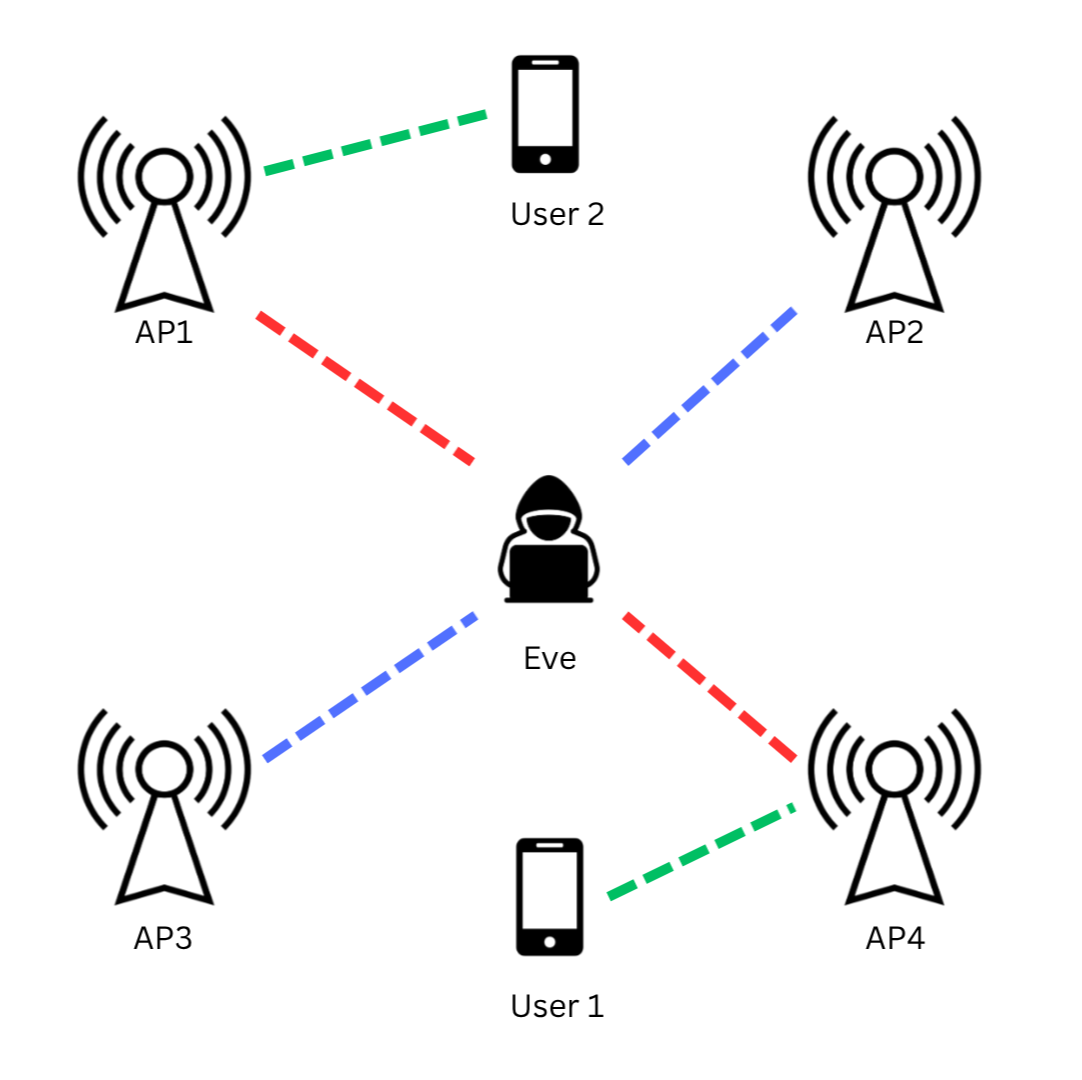
\includegraphics[width=\columnwidth]{AP1.png}
    \caption{System model. User 2 receives downlink traffic from AP1, and User 1 receives downlink traffic from AP4 (green dashed lines). Eve intercepts this traffic from both data-transmitting APs (red dashed lines). AP2 and AP3, unassociated with either user, transmit artificial noise toward Eve (blue dashed lines).}
    \label{fig:system_model}
\end{figure}

\subsection{Propagation Model}

We adopt the Friis free-space path loss model \cite{rappaport}. The received power at node $u$ from AP $n$ transmitting at power $p_n$ is

\begin{equation}
p^r_{n,u}=p_n\cdot\left(\frac{\lambda}{4\pi}\right)^2\cdot d_{n,u}^{-\gamma}
\end{equation}

where $d_{n,u}$ is the Euclidean distance between AP $n$ and node $u$, $\lambda=0.125$ m at $f=2.4$ GHz, and $\gamma=2.0$. The noise floor is $N_0=3.162\times10^{-12}$ W ($-85$ dBm), matching \cite{hoseini}. Antenna gains $G_t=G_r=1$ throughout.

\subsection{SINR and Channel Capacity}

The SINR at legitimate user $k$, served by AP $\alpha_k$, is

\begin{equation}
SINR_k=
\frac{p^r_{\alpha_k,k}}
{\sum_{n\neq\alpha_k}p^r_{n,k}+N_0}
\end{equation}

Every AP not serving user $k$ --- whether it is serving a different user or transmitting jamming noise --- contributes to the interference term in (2), since the physical channel does not distinguish a jamming signal from an ordinary data transmission on the same band. The Shannon capacity of the link between AP $n$ and user $k$ is

\begin{equation}
C_{n,k}=\log_2(1+SINR_{n,k})
\end{equation}

The capacity of the channel between AP $n$ and eavesdropper $j$ is computed identically, evaluated at Eve's coordinates:

\begin{equation}
C^e_{n,j}=\log_2(1+SINR_{n,j})
\end{equation}

All capacities are reported in bits/s/Hz (bps/Hz).

\subsection{Secrecy Capacity}

Assuming the eavesdropper wiretapping AP $n$ achieves the highest capacity among all $J$ eavesdroppers,

\begin{equation}
C^e(n)=\max\{C^e_{n,j}:j=1,\dots,J\}
\end{equation}

the secrecy capacity for user $k$ associated with AP $\alpha_k$ is the non-negative excess of the legitimate link's capacity over the eavesdropper's \cite{wyner,gaussian,broadcast}:

\begin{equation}
C_s(u_k,\alpha_k)=
\left[C_{\alpha_k,k}-C^e(\alpha_k)\right]^+
\end{equation}

where $[x]^+=\max\{x,0\}$. A positive $C_s$ implies the existence of a coding scheme under which the eavesdropper cannot decode the message regardless of its computational capability \cite{wyner}.

\subsection{Problem Formulation}

The joint optimization over user association $A=[\alpha_1,\dots,\alpha_K]$ and transmit power $P=[p_1,\dots,p_N]$ is

\begin{equation}
\Psi:\max_{P,A}\sum_{k=1}^{K}C_s(u_k,\alpha_k),
\quad
\text{s.t. }0\leq p_n\leq P_{\max}
\end{equation}

Problem (7) is non-convex, since $C_s$ is a difference of two logarithmic SINR terms, and jointly optimizing $P$ and $A$ compounds this difficulty. Following \cite{hoseini}, we decouple it into two subproblems. Each user $u_k$ is first associated with the AP that maximizes secrecy capacity under a reference power vector $P_{\text{ref}}$:

\begin{equation}
\alpha_k=
\arg\max_n
C_s(u_k,n)\big|_{P=P_{\text{ref}}}
\end{equation}

In \cite{hoseini}, $P_{\text{ref}}$ is fixed to uniform maximum power ($P_{\text{ref}}=\mathbf{1}\cdot P_{\max}$) and (8) is evaluated once at the start of the episode, before the agent selects its actual power vector. We revisit this choice of $P_{\text{ref}}$ in Section~\ref{sec:association}. With association $A$ fixed, the remaining power allocation problem

\begin{equation}
\Phi:\max_{P}\sum_{k=1}^{K}C_s(u_k,\alpha_k),
\quad
\text{s.t. }0\leq p_n\leq P_{\max}
\end{equation}

remains non-convex and is solved with deep reinforcement learning.

\begin{table}[t]
\caption{Simulation Parameters}
\centering
\begin{tabular}{|l|l|}
\hline
\textbf{Parameter} & \textbf{Value} \\
\hline
Area & $50\text{m} \times 50\text{m}$ \\
APs $(N)$ & 4 \\
Users $(K)$ & 2 \\
Eavesdroppers $(J)$ & 1 \\
Frequency & 2.4 GHz \\
Wavelength $\lambda$ & 0.125 m \\
Path loss exponent $\gamma$ & 2.0 \\
Noise floor $N_0$ & $-85$ dBm \\
Max transmit power $P_{\max}$ & 1.0 W \\
Episode type & Single-step \\
$\sigma$ (training) & $U[0,10]$ m per episode \\
$\rho=\sigma/D_{\max}$, $D_{\max}=50$m & $[0, 0.2]$ \\
Worst-case samples $M$ & 5 \\
\hline
\end{tabular}
\end{table}

\section{Literature Review}
\label{sec:litreview}

\subsection{Foundations and the Recurring CSI-Uncertainty Gap}

Secrecy without encryption is possible whenever the legitimate channel statistically dominates the eavesdropper's, a result established by Wyner \cite{wyner} and specialized to the Gaussian channel by Leung-Yan-Cheong and Hellman, whose closed-form $C_s = C_M - C_{MW}$ is the direct algebraic ancestor of (6); they were also the first to observe in print that a modest SNR gap on the eavesdropper's channel is enough to lose secrecy entirely \cite{gaussian}, flagging CSI uncertainty as a practical vulnerability as early as 1978. Csiszár and Körner extended the framework to broadcast channels \cite{broadcast}. Tekin and Yener generalized the wire-tap channel to multiple simultaneous transmitters, showing that undecoded messages from other users incidentally jam the eavesdropper --- the information-theoretic ancestor of cooperative jamming --- and explicitly proposed a "worst case system design, considering the boundary of the secure area" as future work whenever the eavesdropper's exact position is unknown \cite{tekin}; to our knowledge this proposal was not concretely realized until the present work. Dong et al. formalized cooperative jamming via dedicated relays under full global CSI and named optimization under only statistical eavesdropper CSI as their own open problem \cite{dong}. These three papers, spanning 1978 to 2010, independently and repeatedly name imperfect eavesdropper CSI as unresolved.

\subsection{Deep Reinforcement Learning, SAC, and the Hoseini Baseline}

DRL was established as a general tool for wireless resource management before its application to jamming: Luong et al. survey DRL across access, caching, and network security \cite{luong}; Nasir and Guo show distributed multi-agent DQN power control tolerant of delayed, local-only CSI \cite{nasir}; and Li et al. apply DQN to network slicing \cite{slice}. None address secrecy, but together they establish DRL as proven for power and resource control under partial information. We adopt Soft Actor-Critic \cite{sac1}, the same algorithm as \cite{hoseini}; its companion paper's automatic temperature tuning, which reformulates the entropy coefficient as a dual variable, is the exact mechanism our $\alpha_{\text{base}}$ is drawn from \cite{sac2}, and the original paper's identification of reward scale as SAC's one sensitive hyperparameter \cite{sac1} is a sensitivity we revisit in Section~\ref{sec:results}.

Hoseini et al. is the direct foundation of this work: an MDP with state $S=\{L_{AP},L_u,L_e\}$, including Eve's exact location, and SAC-based power allocation outperforming fixed-power and non-adaptive AP-selection baselines across six scenarios \cite{hoseini}. Critically, their own fifth scenario shows sum secrecy capacity \emph{decreasing} when APs are added, which they diagnose themselves as a consequence of computing AP association once under a fixed uniform-power assumption and never revisiting it --- an observed failure, not a hypothesized one, that motivates the correction in Section~\ref{sec:association}. Closely related recent work applies SAC to jamming-adjacent problems: Liu et al. jointly tune transmitter and friendly-jammer power for covert communication \cite{covertsac}; Xing et al. jointly learn UAV association, trajectory, and jamming power to maximize the \emph{minimum} secrecy rate across users, evidence that joint association-and-power learning is tractable \cite{xing24}; Tripathi et al. justify full eavesdropper CSI specifically for active or monitored adversaries \cite{tripathi24}, scoping our own contribution to the complementary passive case; and Zhao et al. offer a \emph{certified} robustness guarantee for the mirror-image anti-jamming problem \cite{zhao25}, a categorically stronger guarantee than our own empirical sampling, which we scope against explicitly in Section~\ref{sec:results}.

\subsection{Grounding the Worst-Case Reward}

Our reward's theoretical grounding draws on three sources. Wang, Kallus, and Sun formalize the Conditional Value-at-Risk objective and show that as its risk parameter $\tau \to 0$, CVaR converges to the single worst-case outcome \cite{cvar}; $R^*$, a minimum over $M=5$ samples, is precisely a finite-sample approximation of this small-$\tau$ regime, without inheriting their tabular regret guarantees. Tanabe et al.'s M2TD3 \emph{learns} the worst-case condition adversarially rather than sampling it \cite{m2td3} --- more rigorous, and a candidate future direction should $M=5$ prove insufficient. Lanier et al. show that uncertainty sets defined too broadly produce needlessly conservative policies \cite{farr}, directly justifying our choice to bound $\sigma \in [0,10]$m rather than train against unbounded uncertainty. Chen et al. justify the complementary half of our design: uniform per-episode sampling of $\sigma$ transfers to held-out conditions under domain randomization theory \cite{domainrand} --- distinct from, and not a substitute for, the worst-case minimization \emph{given} $\sigma$ that CVaR and M2TD3 justify.

\subsection{Reflective Surfaces and Statistical-CSI Alternatives}

A parallel line of work secures communication via reconfigurable reflecting surfaces rather than jamming power. Mukherjee and Swindlehurst's artificial-noise beamforming needs no eavesdropper CSI but has a hard analytical breaking point under large channel mismatch \cite{mukherjee}, contrasting with UA-SAC's empirical rather than certified robustness; Wang et al.'s outage-robust MISO precoding \cite{wang} and Liu et al.'s survey of compound wiretap channels \cite{liu} contribute the same worst-case-over-a-set methodology from an earlier, non-RL lineage. Yang et al. jointly optimize active/passive beamforming under CSI staleness and critique jamming for its extra power cost \cite{yang} --- a fair critique we accept, since CFJ needs no new hardware where IRS does. Xiao et al. \cite{starris} and Zhou et al. \cite{zhou26} secure networks under genuinely unknown eavesdropper location via large-system asymptotics; Zhou et al.'s finding that positional uncertainty produces geometry-\emph{dependent} angular error is a direct, unresolved critique of our own geometry-blind global scalar $\rho$, named explicitly in Section~\ref{sec:conclusion}. Miao et al. solve imperfect-CSI RIS beamforming via model-driven deep unfolding \cite{miao26}, a paradigm requiring a differentiable structure our joint association/power/interference problem lacks; Niu et al.'s survey notes CSI-free artificial-noise designs are computationally expensive at inference \cite{ansurvey}, a cost UA-SAC avoids since a trained policy's inference is one forward pass. Bui et al. resolve unknown-Eve secure ISAC via radar echo feedback \cite{bui26}, a sensing modality ordinary Wi-Fi APs lack; Abughalwa et al. report a Jain's fairness index near 1.0 for a max-min secrecy objective versus 0.2--0.3 for sum-rate maximization \cite{abughalwa25}, quantified evidence that worst-case objectives produce materially different behavior than average-case ones.

\subsection{Infrastructure and an Unresolved Assumption Conflict}

Bouhafs et al.'s Wi-5 architecture provides per-AP power control via open APIs \cite{wifi5}, the deployability foundation a centralized UA-SAC controller assumes. A later paper by overlapping authors, however, builds a secrecy-aware AP-\emph{selection} algorithm on the same architecture whose adversary model assumes Eve's location \emph{is} known to the network, citing prior AP-based detection capability \cite{spectrum} --- a direct conflict with this work's premise that we address rather than ignore: their assumption presupposes a separate, trusted detection layer; our contribution targets the case where that layer is unavailable or untrusted, the more conservative threat model for a genuinely passive adversary.

\section{Proposed Methodology}
\label{sec:methodology}

We solve (9) with SAC \cite{sac1,sac2}, extending \cite{hoseini} in two independent respects: UA-SAC (Sections~\ref{sec:layer1}--\ref{sec:layer3}) removes the perfect-eavesdropper-location assumption from the reward and state, and the association correction (Section~\ref{sec:association}) removes a documented flaw from the association step defined in (8). The two are additive and orthogonal --- one changes what the reward is scored against, the other changes how association is computed given a power vector --- and both are active in every result reported in Section~\ref{sec:results}.

\subsection{Layer 1 --- Worst-Case Robust Reward}
\label{sec:layer1}

Where \cite{hoseini} computes the reward using the eavesdropper's single true position, we compute the minimum secrecy achieved across $M$ independently sampled candidate positions drawn around the true location:

\begin{equation}
\hat{E}_i=
\text{clip}(E+\epsilon_i,0,D_{\max}),
\quad
\epsilon_i\sim\mathcal{N}(0,\sigma^2I_2)
\end{equation}

\begin{equation}
R^*=
\min_{i=1}^{M}
\sum_{k=1}^{K}
\left[
C(AP_{\alpha_k}\rightarrow u_k|P)
-
\max_j C(AP_{\alpha_k}\rightarrow e_j|P,\hat{E}_i)
\right]^+
\end{equation}

As discussed in Section~\ref{sec:litreview}, $R^*$ is a finite-sample approximation of a small-$\tau$ CVaR objective \cite{cvar}, not a certified worst-case bound \cite{zhao25}; we return to this scoping in Section~\ref{sec:results}.

\subsection{Layer 2 --- Uncertainty-Augmented State}
\label{sec:layer2}

We introduce a normalized uncertainty ratio $\rho=\sigma/D_{\max}$, and augment the state with it so a single policy can condition its behavior on the current confidence level of the eavesdropper location estimate:

\begin{equation}
s^*=
[
x_1,y_1,\dots,x_4,y_4
\mid
x_{u_1},y_{u_1},x_{u_2},y_{u_2}
\mid
\hat{e}_x,\hat{e}_y
\mid
\rho
]
\in\mathbb{R}^{15}
\end{equation}

Each episode draws $\sigma \sim U[0,10]\text{m}$ independently, so that $\rho \in [0, 0.2]$ over the course of training --- we correct here an inconsistency in an earlier draft of this work that reported the theoretical range $\rho \in [0,1]$; the practical training range determined by $\sigma_{\max}=10$m and $D_{\max}=50$m is $[0,0.2]$. Per Chen et al. \cite{domainrand}, uniform sampling of $\sigma$ across episodes is the mechanism that lets a single policy generalize across all uncertainty levels, distinct from the worst-case minimization within a given $\sigma$ described in Section~\ref{sec:layer1}. The action space is the continuous transmit power vector $P=[p_1,p_2,p_3,p_4]$, $p_n \in [0,P_{\max}]$.

\subsection{Layer 3 --- Uncertainty-Scaled Entropy (Ablated)}
\label{sec:layer3}

We additionally investigated scaling SAC's entropy coefficient with $\rho$,

\begin{equation}
\alpha_{\text{eff}}(\rho)=
\alpha_{\text{base}}
\cdot
(1+\beta\cdot\rho)
\end{equation}

with the intent of broadening exploration when the eavesdropper location estimate is unreliable. We report this modification here for completeness of the design space explored, but as detailed in Section~\ref{sec:results}, a controlled ablation found this layer to be, at best, of marginal and inconsistent benefit, and it is disabled ($\beta=0$) in the model we report as our final result.

\subsection{Power-Aware Association Correction}
\label{sec:association}

The association rule in (8) requires a reference power vector $P_{\text{ref}}$ before power allocation has occurred, and \cite{hoseini} resolves this circularity by fixing $P_{\text{ref}} = \mathbf{1}\cdot P_{\max}$ --- a fair, neutral choice for breaking the dependency, and not itself the source of error. The error, which \cite{hoseini} documents empirically in their own scenario 5, is that this association is computed once, under this fictitious reference, and never revisited once the agent's real power vector $P$ is known, even though $P$ is typically very different from $\mathbf{1}\cdot P_{\max}$.

We correct this by recomputing (8) using the agent's actual chosen power vector, immediately before scoring the reward, rather than the fixed reference:

\begin{equation}
\alpha_k=
\arg\max_n
C_s(u_k,n)\big|_{P=P}
\end{equation}

\textbf{Proposition (weak dominance).} For any fixed power vector $P$, let $A^{\text{fixed}}$ denote the association obtained from (8) under $P_{\text{ref}} = \mathbf{1}\cdot P_{\max}$, and let $A^{P}$ denote the association obtained from (14) using $P$ itself. Then $\sum_k C_s(u_k, \alpha_k^P) \geq \sum_k C_s(u_k, \alpha_k^{\text{fixed}})$.

\emph{Proof sketch.} By construction, $\alpha_k^P = \arg\max_n C_s(u_k,n)|_{P}$ selects, for each user $k$, whichever AP maximizes secrecy capacity under the power vector $P$ that is actually used to score the reward. $\alpha_k^{\text{fixed}}$ is one specific candidate AP inside this same maximization, computed instead using a possibly unrelated reference power vector. Since $\alpha_k^P$ maximizes over the same objective evaluated at the same $P$, it can score no worse than any other candidate, including $\alpha_k^{\text{fixed}}$. $\blacksquare$

The correction requires no change to the agent's action space, network architecture, or reward mechanism; it modifies only when and with what argument (8) is evaluated. We do not conduct a scenario-5-style AP-density sweep to independently isolate this correction's effect in the present work; its contribution is embedded within all headline results reported in Section~\ref{sec:results}, since it is applied uniformly to every system evaluated there.

\subsection{Implementation}

The environment is implemented as a Gymnasium environment (\texttt{env/cfj\_env.py}) and trained with Stable-Baselines3 SAC. Both the perfect-CSI baseline and UA-SAC use identical network architectures --- four hidden layers of widths $[256,128,64,32]$ --- and identical association and propagation mechanics; the only differences between them are the reward, state, and entropy modifications described above. This architecture was chosen after an initial attempt to match \cite{hoseini}'s reported network depth of "nine layers" as a literal nine-weight-layer multilayer perceptron produced measurable training instability (a critic loss that failed to converge and instead rose over the second half of training), consistent with documented findings that deep, unnormalized actor-critic networks exhibit unstable gradients as depth increases \cite{bjorck2021}; we interpret \cite{hoseini}'s reported depth as more plausibly corresponding to a MATLAB layer count that includes activation layers separately from weight layers, and the four-hidden-layer architecture used here is our best-performing reinterpretation of that reported depth. The perfect-CSI baseline was trained for 100{,}000 timesteps, at which point its critic loss had converged; UA-SAC required 300{,}000 timesteps to reach comparable convergence, which we attribute to its training signal being substantially noisier than the baseline's --- every episode draws an independent uncertainty level $\sigma$, the observed state includes a noisy rather than exact eavesdropper position, and the reward itself is a minimum over $M=5$ stochastic samples rather than a single deterministic value. Both models use 4 parallel \texttt{SubprocVecEnv} workers, a replay buffer of 200{,}000 transitions, batch size 256, and learning rate $3\times10^{-4}$.

\section{Results and Discussion}
\label{sec:results}

Evaluation uses 1{,}000 fixed-seed randomized topologies, shared identically across every system compared, so that per-topology paired comparisons are valid. All secrecy figures are computed against each topology's true eavesdropper location; only the state observed by UA-SAC and the perfect-CSI baseline during evaluation is affected by the injected location noise $\sigma$.

\subsection{System Comparison at Maximum Uncertainty}

Table~\ref{table:comparison_sigma10} compares four systems at $\sigma=10$m: Normal Wi-Fi, in which each user associates with the AP offering the highest SINR without regard to the eavesdropper's presence, matching \cite{hoseini}'s definition of this baseline; Single Best AP, in which only each user's serving AP transmits and all other APs remain silent, isolating the value of cooperative jamming itself; the perfect-CSI SAC baseline; and UA-SAC.

\begin{table}[htbp]
\caption{System Comparison at $\sigma = 10$m ($n=1{,}000$ topologies)}
\label{table:comparison_sigma10}
\centering
\begin{tabular}{@{}lccc@{}}
\toprule
\textbf{System} &
\textbf{\begin{tabular}[c]{@{}c@{}}Sum Secrecy \\ (bps/Hz)\end{tabular}} &
\textbf{\begin{tabular}[c]{@{}c@{}}Gain over \\ Normal Wi-Fi\end{tabular}} &
\textbf{\begin{tabular}[c]{@{}c@{}}Secrecy \\ Ratio\end{tabular}} \\
\midrule
Normal Wi-Fi (no PLS)      & 2.26 & ---     & 97\% \\
Single Best AP (no jamming) & 3.68 & +63.0\% & 98\% \\
Baseline SAC (perfect CSI) & 3.98 & +76.2\% & 100\% \\
UA-SAC (ours)              & 4.53 & +100.6\% & 100\% \\
\bottomrule
\end{tabular}
\end{table}

UA-SAC exceeds the perfect-CSI baseline by $13.9\%$ ($4.53$ vs.\ $3.98$ bps/Hz) despite having no access to the eavesdropper's true location at any point during training or evaluation, and exceeds Single Best AP by $23.1\%$, indicating that cooperative jamming under a learned, uncertainty-aware policy provides a genuine benefit over withholding jamming entirely. We verified this comparison is not an artifact of a single favorable evaluation: a paired $t$-test across the 1{,}000 shared topologies gives a mean difference of $0.551$ bps/Hz (UA-SAC $-$ baseline) with standard error $0.055$ and $t=10.04$ at $\sigma=10$m, and $0.584$ with standard error $0.056$ and $t=10.40$ at $\sigma=0$m; UA-SAC exceeds the baseline on $61.6\%$ and $61.8\%$ of individual topologies respectively, so the advantage is genuine at the level of individual network instances and not solely an averaging effect.

\begin{figure}[H]
\centering

\includegraphics[width=1\linewidth]{plot1.png}
\caption{Four-system comparison of sum secrecy capacity at $\sigma=10$m. Secrecy ratio for the same four systems is reported in Table~\ref{table:comparison_sigma10}.}
\label{fig:comparison_bar}
\end{figure}

\subsection{Secrecy Capacity Across the Uncertainty Range}

Fig.~\ref{fig:secrecy_vs_noise} sweeps $\sigma$ from 0 to 10m in 1m increments. UA-SAC exceeds the perfect-CSI baseline at every value of $\sigma$ tested, including $\sigma=0$, where UA-SAC still exceeds the baseline ($4.65$ vs.\ $4.06$ bps/Hz) despite the baseline having been trained specifically and exclusively for this condition. We interpret this carefully rather than attribute it solely to robustness against uncertainty: since the advantage is present even at zero uncertainty, and the two curves in Fig.~\ref{fig:secrecy_vs_noise} decline at broadly similar rates rather than diverging as $\sigma$ increases, the more precise characterization of UA-SAC's advantage is that it learns a higher-performing power allocation policy overall, evaluated across the full range of uncertainty conditions it was trained on, rather than a policy whose \emph{rate of degradation} under increasing uncertainty is specifically superior to the baseline's. Both non-RL references are included for scale: Normal Wi-Fi and Single Best AP are, by construction, invariant to the injected observation noise $\sigma$, since neither uses any eavesdropper information at all.

\begin{figure}[H]
\centering

\includegraphics[width=1\linewidth]{plot2_secrecy_vs_noise.png}
\caption{Mean sum secrecy capacity vs.\ eavesdropper location uncertainty $\sigma$, all four systems, 1{,}000 shared topologies per point.}
\label{fig:secrecy_vs_noise}
\end{figure}

\subsection{Normalized Degradation}

Fig.~\ref{fig:robustness} normalizes each RL agent's own $\sigma=0$ performance to 100\%, isolating the \emph{shape} of degradation independent of the two systems' different absolute capacities. UA-SAC retains $97.5\%$ of its $\sigma=0$ performance at $\sigma=10$m; the baseline retains $97.9\%$. We report this without adjustment: on this specific normalized-degradation metric, UA-SAC does not outperform the baseline, and in fact degrades marginally more in proportional terms. This is consistent with the interpretation in the previous subsection --- UA-SAC's advantage lies in the absolute level of secrecy capacity achieved across the uncertainty range, not in a shallower degradation slope, and we do not claim the latter.

\begin{figure}[H]
\centering

\includegraphics[width=1\linewidth]{plot3_robustness.png}
\caption{Secrecy capacity normalized to each agent's own $\sigma=0$ performance (100\%).}
\label{fig:robustness}
\end{figure}

\subsection{Training Convergence}

Fig.~\ref{fig:training_convergence} shows UA-SAC's worst-case training reward $R^*$ over 300{,}000 episodes. $R^*$ rises from approximately 2.0 bps/Hz to approximately 3.4--3.5 bps/Hz, with substantial episode-to-episode variance attributable to the randomized $\sigma$ and stochastic $M$-sample minimum described in Section~\ref{sec:layer1} --- easy episodes ($\rho \approx 0$) and hard episodes ($\rho \approx 0.2$) are interleaved throughout training. The curve is monotonically increasing without evidence of divergence, consistent with legitimate convergence rather than the instability observed in our earlier nine-weight-layer architecture attempt (Section~\ref{sec:methodology}).

\begin{figure}[H]
    \centering
    
\includegraphics[width=\columnwidth]{plot5_convergence.png}
    \caption{UA-SAC training convergence: worst-case reward $R^*$ versus training episode.}
    \label{fig:training_convergence}
\end{figure}

\subsection{Ablation: Uncertainty-Scaled Entropy}

We evaluated the effect of Layer 3 (Section~\ref{sec:layer3}) with a controlled ablation: an otherwise identical UA-SAC model trained with $\beta=1$ for the same 300{,}000 timesteps as the $\beta=0$ model reported above, holding architecture, environment, and every other hyperparameter fixed. Table~\ref{table:ablation} reports both against the perfect-CSI baseline and against each other.

\begin{table}[htbp]
\caption{Entropy-Scaling Ablation ($n=1{,}000$ topologies)}
\label{table:ablation}
\centering
\begin{tabular}{@{}lcc@{}}
\toprule
\textbf{Comparison} & $\sigma=0$m & $\sigma=10$m \\
\midrule
UA-SAC ($\beta=0$) vs.\ baseline: mean diff (t, win\%) & $0.58$ (10.40, 61.8\%) & $0.55$ (10.04, 61.6\%) \\
UA-SAC ($\beta=0$) vs.\ UA-SAC ($\beta=1$): mean diff (t, win\%) & $0.10$ (2.27, 51.4\%) & $0.13$ (3.00, 54.4\%) \\
\bottomrule
\end{tabular}
\end{table}

Both variants of UA-SAC substantially exceed the perfect-CSI baseline at both training budgets tested, which indicates that the additional training budget (300{,}000 vs.\ 100{,}000 timesteps), not the entropy-scaling mechanism, is the primary factor separating UA-SAC's earlier underperformance (observed at 100{,}000 timesteps in preliminary experiments not reported in detail here) from its reported result. Between the two UA-SAC variants, $\beta=0$ outperforms $\beta=1$ at both uncertainty levels, but the effect is markedly weaker than the UA-SAC-versus-baseline gap: the win rate across individual topologies is $51.4\%$ and $54.4\%$, close to even, and while $t=3.00$ at $\sigma=10$m clears a conventional significance threshold, $t=2.27$ at $\sigma=0$m is only marginal. We report $\beta=0$ as our final configuration on the strength of this directionally consistent but modest advantage, and we are explicit that this specific finding rests on a single trained instance of each configuration rather than a multi-seed replication; we consider it suggestive rather than conclusive, and note it as an open question for further verification in Section~\ref{sec:conclusion}.

\section{Conclusion and Future Work}
\label{sec:conclusion}

This paper addressed the assumption, common to Hoseini et al.'s DRL-based cooperative jamming formulation and, to our knowledge, every subsequent DRL-CFJ formulation, that a passive eavesdropper's exact location is available to the network controller. We proposed UA-SAC, which replaces this assumption with a worst-case reward computed over sampled eavesdropper positions and a normalized uncertainty variable appended to the observed state, and we identified and corrected a specific, previously undiagnosed consequence of a limitation Hoseini et al. report in their own results: their AP-association step is computed once under a fictitious uniform-power reference and never revisited, which we correct with a change we prove is weakly dominant over the original heuristic. Evaluated over 1{,}000 shared topologies, UA-SAC achieves a $13.9\%$ improvement in sum secrecy capacity over a perfect-CSI SAC baseline trained under identical conditions, an effect that is statistically robust ($t=10.04$, $n=1{,}000$) and present at the majority of individual network topologies, not only on average.

Several limitations bound the scope of this contribution and motivate future work. First, our uncertainty signal $\rho$ is a single global scalar, identical regardless of the eavesdropper's position relative to the APs; Zhou et al.'s finding that positional uncertainty produces geometry-dependent angular error \cite{zhou26} suggests a geometry-aware uncertainty representation could improve on this. Second, UA-SAC's robustness is empirical, established via $M=5$ Monte Carlo samples rather than a certified bound; approaches such as Zhao et al.'s interval-bound-propagation method \cite{zhao25} or Tanabe et al.'s adversarially-learned worst case \cite{m2td3} offer stronger guarantees at the cost of substantially greater implementation complexity, and remain open directions if $M=5$ sampling proves insufficient at larger scale. Third, our association correction (Section~\ref{sec:association}) leaves association a fixed, non-learned rule reactive to the agent's power output, rather than a decision the agent learns jointly with power allocation; Xing et al. demonstrate that joint association-and-power learning via DRL is tractable in a related secure UAV setting \cite{xing24}, and extending UA-SAC similarly --- which would require a hybrid discrete-continuous action space --- is, to our knowledge, still the concrete integration Hoseini et al. themselves proposed as future work and which neither their system nor ours has yet realized. Fourth, the entropy-scaling ablation in Section~\ref{sec:results} rests on a single training run per configuration; a multi-seed replication would be needed to confirm the modest advantage we report for $\beta=0$ is not run-to-run variance. Finally, as in \cite{hoseini}, our eavesdropper and node positions are redrawn independently each episode rather than moving continuously across episodes, and our channel model is free-space Friis path loss rather than a fading channel; extending UA-SAC to mobile nodes and to multipath/shadowing/Rayleigh-fading conditions, and validating the resulting policy on physical Wi-Fi hardware, are natural next steps toward deployment.

\bibliographystyle{IEEEtran}

\begin{thebibliography}{35}

\bibitem{wyner}
A. D. Wyner, ``The wire-tap channel,'' \emph{Bell Syst. Tech. J.}, vol. 54, no. 8, pp. 1355--1387, 1975.

\bibitem{gaussian}
S. K. Leung-Yan-Cheong and M. E. Hellman, ``The Gaussian wire-tap channel,'' \emph{IEEE Trans. Inf. Theory}, vol. 24, no. 4, pp. 451--456, 1978.

\bibitem{broadcast}
I. Csisz\'ar and J. K\"orner, ``Broadcast channels with confidential messages,'' \emph{IEEE Trans. Inf. Theory}, vol. 24, no. 3, pp. 339--348, 1978.

\bibitem{tekin}
E. Tekin and A. Yener, ``The Gaussian multiple access wire-tap channel,'' \emph{IEEE Trans. Inf. Theory}, vol. 54, no. 12, pp. 5747--5755, Dec. 2008.

\bibitem{dong}
L. Dong, Z. Han, A. P. Petropulu, and H. V. Poor, ``Improving wireless physical layer security via cooperating relays,'' \emph{IEEE Trans. Signal Process.}, vol. 58, no. 3, pp. 1875--1888, Mar. 2010.

\bibitem{luong}
N. C. Luong, D. T. Hoang, S. Gong, D. Niyato, P. Wang, Y.-C. Liang, and D. I. Kim, ``Applications of deep reinforcement learning in communications and networking: A survey,'' \emph{IEEE Commun. Surveys Tuts.}, vol. 21, no. 4, pp. 3133--3174, 2019.

\bibitem{nasir}
Y. S. Nasir and D. Guo, ``Multi-agent deep reinforcement learning for dynamic power allocation in wireless networks,'' \emph{IEEE J. Sel. Areas Commun.}, vol. 37, no. 10, pp. 2239--2250, Oct. 2019.

\bibitem{slice}
R. Li, Z. Zhao, Q. Sun, C.-L. I, C. Yang, X. Chen, M. Zhao, and H. Zhang, ``Deep reinforcement learning for resource management in network slicing,'' \emph{IEEE Access}, vol. 6, pp. 74429--74441, 2018.

\bibitem{sac1}
T. Haarnoja, A. Zhou, P. Abbeel, and S. Levine, ``Soft actor-critic: Off-policy maximum entropy deep reinforcement learning with a stochastic actor,'' in \emph{Proc. ICML}, PMLR vol. 80, 2018, pp. 1856--1865.

\bibitem{sac2}
T. Haarnoja, A. Zhou, K. Hartikainen, G. Tucker, S. Ha, J. Tan, V. Kumar, H. Zhu, A. Gupta, P. Abbeel, and S. Levine, ``Soft actor-critic algorithms and applications,'' arXiv:1812.05905, 2018.

\bibitem{mukherjee}
A. Mukherjee and A. L. Swindlehurst, ``Robust beamforming for security in MIMO wiretap channels with imperfect CSI,'' \emph{IEEE Trans. Signal Process.}, vol. 59, no. 1, pp. 351--361, Jan. 2011.

\bibitem{wang}
K.-Y. Wang, A. M.-C. So, T.-H. Chang, W.-K. Ma, and C.-Y. Chi, ``Outage constrained robust transmit optimization for multiuser MISO downlinks: Tractable approximations by conic optimization,'' \emph{IEEE Trans. Signal Process.}, vol. 62, no. 21, pp. 5690--5705, Nov. 2014.

\bibitem{yang}
H. Yang, Z. Xiong, J. Zhao, D. Niyato, L. Xiao, and Q. Wu, ``Deep reinforcement learning based intelligent reflecting surface for secure wireless communications,'' \emph{IEEE Trans. Wireless Commun.}, vol. 20, no. 1, pp. 375--388, Jan. 2021.

\bibitem{wifi5}
F. Bouhafs, M. Mackay, A. Raschell\`a, Q. Shi, F. den Hartog, J. Sald\'ana, R. Munilla, J. Ruiz-Mas, J. Fern\'andez-Navajas, J. Almodovar, and N. van Adrichem, ``Wi-5: A programming architecture for unlicensed frequency bands,'' \emph{IEEE Commun. Mag.}, 2018.

\bibitem{spectrum}
F. Bouhafs, F. den Hartog, A. Raschell\`a, M. Mackay, Q. Shi, and S. Sinanovic, ``Realizing physical layer security in large wireless networks using spectrum programmability,'' in \emph{Proc. IEEE Globecom Workshops}, 2020.

\bibitem{hoseini}
S. A. Hoseini, F. Bouhafs, N. Aboutorab, P. Sadeghi, and F. den Hartog, ``Cooperative jamming for physical layer security enhancement using deep reinforcement learning,'' in \emph{Proc. IEEE Globecom Workshops}, 2023, pp. 1838--1843.

\bibitem{rappaport}
T. S. Rappaport, \emph{Wireless Communications: Principles and Practice}, 2nd ed. Prentice Hall, 2002.

\bibitem{liu}
Y. Liu, H.-H. Chen, and L. Wang, ``Physical layer security for next generation wireless networks: Theories, technologies, and challenges,'' \emph{IEEE Commun. Surveys Tuts.}, vol. 19, no. 1, pp. 347--376, 2017.

\bibitem{zhao25}
H. Zhao, Z. Li, J. Si, R. Huang, H. Hu, T. Q. S. Quek, and N. Al-Dhahir, ``DRL-based robust multi-timescale anti-jamming approaches under state uncertainty,'' \emph{IEEE Trans. Cogn. Commun. Netw.}, 2025, arXiv:2511.03305.

\bibitem{covertsac}
Y. Liu, J. Wen, Z. Zhang, K. Zhu, Y. Zhang, J. Nie, and J. Kang, ``Learning-based power control for secure covert semantic communication,'' arXiv:2407.07475, 2024.

\bibitem{m2td3}
T. Tanabe, R. Sato, K. Fukuchi, J. Sakuma, and Y. Akimoto, ``Max-min off-policy actor-critic method focusing on worst-case robustness to model misspecification,'' in \emph{Proc. NeurIPS}, 2022, arXiv:2211.03413.

\bibitem{farr}
J. B. Lanier, S. McAleer, P. Baldi, and R. Fox, ``Feasible adversarial robust reinforcement learning for underspecified environments,'' in \emph{Proc. NeurIPS}, 2022, arXiv:2207.09597.

\bibitem{domainrand}
X. Chen, J. Hu, C. Jin, L. Li, and L. Wang, ``Understanding domain randomization for sim-to-real transfer,'' in \emph{Proc. ICLR}, 2022, arXiv:2110.03239.

\bibitem{cvar}
K. Wang, N. Kallus, and W. Sun, ``Near-minimax-optimal risk-sensitive reinforcement learning with CVaR,'' in \emph{Proc. ICML}, 2023, arXiv:2302.03201.

\bibitem{xing24}
Z. Xing, Y. Qin, C. Du, W. Wang, and Z. Zhang, ``Deep reinforcement learning-driven jamming-enhanced secure unmanned aerial vehicle communications,'' \emph{Sensors}, vol. 24, no. 22, article 7328, Nov. 2024.

\bibitem{tripathi24}
S. Tripathi, C. Kundu, A. Yadav, A. Bansal, H. Claussen, and L. Ho, ``Joint transmit and jamming power optimization for secrecy in energy harvesting networks: A reinforcement learning approach,'' arXiv:2407.17435, 2024.

\bibitem{miao26}
R. Miao, Z. Song, Y. Li, X. Li, L. Liu, G. Shao, and B. Wang, ``RIS-aided physical layer security with imperfect CSI: A robust model-driven deep learning approach,'' \emph{Entropy}, vol. 28, no. 4, article 457, Apr. 2026.

\bibitem{zhou26}
C. Zhou, C. You, C. Zhou, C. Xing, and J. Zhang, ``Near-field physical layer security: Robust beamforming under location uncertainty,'' \emph{IEEE Trans. Wireless Commun.}, vol. 25, pp. 17384--17398, 2026, arXiv:2601.13549.

\bibitem{starris}
H. Xiao, X. Hu, A. Li, W. Wang, and K. Yang, ``Robust full-space physical layer security for STAR-RIS-aided wireless networks: Eavesdropper with uncertain location and channel,'' \emph{IEEE Trans. Wireless Commun.}, vol. 24, pp. 7206--7220, 2025, arXiv:2503.12233.

\bibitem{ansurvey}
H. Niu, Y. Xiao, X. Lei, J. Chen, Z. Xiao, M. Li, and C. Yuen, ``A survey on artificial noise for physical layer security: Opportunities, technologies, guidelines, advances, and trends,'' arXiv:2507.06500, 2025.

\bibitem{bui26}
B. M. Tuan, V.-D. Nguyen, D. N. Nguyen, N. L. Trung, N. V. Huynh, D. T. Hoang, M. Krunz, and E. Dutkiewicz, ``Deep learning-driven friendly jamming for secure multicarrier ISAC under channel uncertainty,'' arXiv:2603.05062, Mar. 2026.

\bibitem{abughalwa25}
M. Abughalwa, D. N. Nguyen, D. T. Hoang, T. X. Vu, E. Dutkiewicz, and S. Chatzinotas, ``Secure communications for all users in low-resolution IRS-aided systems under imperfect and unknown CSI,'' arXiv:2504.05048, Apr. 2025.

\bibitem{bjorck2021}
J. Bj\"orck, C. P. Gomes, and K. Q. Weinberger, ``Towards deeper deep reinforcement learning,'' arXiv:2106.01151, 2021.

\end{thebibliography}

\end{document}
